\documentclass[12pt, leqno]{article} %% use to set typesize 
\usepackage{amsfonts}
\usepackage{amsmath}
\usepackage{fancyhdr}
\usepackage{hyperref}
\usepackage{tikz}
\usepackage{pgfplots}
\usepackage{listings}

\newcommand{\bbR}{\mathbb{R}}
\newcommand{\bbC}{\mathbb{C}}

\newcommand{\hdr}[2]{
  \pagestyle{fancy}
  \lhead{Bindel, Spring 2015}
  \rhead{Numerical Analysis (CS 4220)}
  \fancyfoot{}
  \begin{center}
    {\large{\bf #1}} \\
    Due: #2
  \end{center}
  \lstset{language=matlab,columns=flexible}
}

\newcommand{\phdr}[1]{
  \pagestyle{fancy}
  \lhead{Bindel, Spring 2015}
  \rhead{Numerical Analysis (CS 4220)}
  \fancyfoot{}
  \begin{center}
    {\large{\bf #1}}
  \end{center}
  \lstset{language=matlab,columns=flexible}
}


\begin{document} \phdr{Proj 3: MEMS Madness}

\section{Introduction}

Micro-Electro-Mechanical Systems (MEMS) are tiny coupled-physics
systems that are often built using the same basic processes one uses
to make integrated circuits.  At characteristic length scales on the
order of microns (millionths of a meter), the physics of these devices
are still predominantly classical, but the dominant forces might be
different than what you would expect.  For example, electrostatic
attraction can be an incredibly strong force at these scales, and is
often used to drive motion.

You are provided with a small finite element code to simulate the
displacement of a cantilever beam suspended over an electrode; the
geometry is shown in Figure~\ref{fig:beam}.  The beam and the
electrode are at different voltages, and so attract each other;
but elastic forces resist that attraction.  The basic force balance
equation is
\[
  Ku = f_e(u, V),
\]
where $K$ is a positive definite stiffness matrix and $f_e$ is the
electrostatic force for a given displacement and voltage.

The electrostatic forces tend to pull the beam toward the electrode,
and scale like with $(g+u)^2$, where $g$ is the initial gap and $u$ is
the displacement.  The elastic restoring forces, in contrast, scale
linearly with $u$.  Hence, at some critical voltage, the electrostatic
forces become so strong that the elastic forces cannot balance them,
and the system becomes unstable.  At this point, the beam is ``pulled
in'' to the electrode underneath.

\begin{figure}
  \begin{center}
  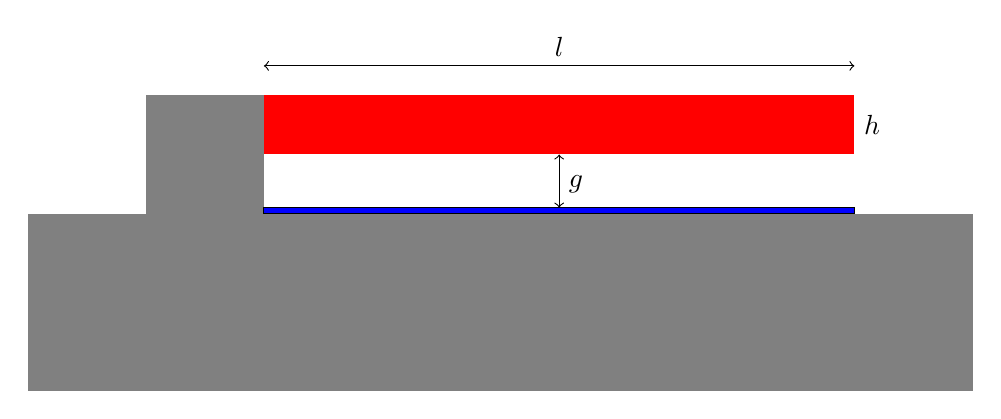
\begin{tikzpicture}[scale=0.75]
    \fill[red] (0,1cm) rectangle (10cm,2cm);
    \fill[black!50] (-2,0cm) rectangle (0cm,2cm);
    \fill[black!50] (-4,0cm) rectangle (12cm,-3cm);
    \draw[fill=blue] (0,0) rectangle (10cm,1mm);
    \node[right] at (10cm,15mm) {$h$};
    \draw[<->] (5cm,1mm) -- (5cm,1cm);
    \draw[<->] (0,25mm) -- (10cm,25mm);
    \node[right] at (5cm,5mm) {$g$};
    \node[above] at (5cm,25mm) {$l$};
  \end{tikzpicture}
  \end{center}
  \caption{Cantilever beam gap-closing actuator.  A potential
    difference between the beam (red) and an electrode along
    the substrate (blue) causes the beam to be pulled down.}
  \label{fig:beam}
\end{figure}

% 1. Solve via fixed point + continuation; how far before failure?
% 2. Solve via Newton + continuation; how far before failure?
% 3. Use tip displacement as parameter and track voltage; plot tip vs V
% 4. Extended system to find the bifurcation point
% 5. Bonus: extrapolation

\section{The approaches}

\subsection{Fixed point iteration}

The {\tt gap\_solve\_fpV} code solves for the deflection in the model
problem using the fixed point iteration
\[
  K u^{(k+1}) = f_e(u^{(k)}; V)
\]
where $f_e$ denotes the electrostatic force vector.  The driver
{\tt gap\_demo} shows how this code is used.

\begin{enumerate}
\item Plot the residual error versus iteration count.  Does this look
  like a linearly convergent iteration?
  
\item Write a new script, {\tt gap\_continuer0} that uses this fixed
  point iteration to solve the equation for voltages starting at $V =
  0$ and going up to $V = 10$ (past the pull-in voltage).  Use a
  continuation strategy in which the initial guess for $u$ at each
  voltage is the equilbrium solution for the previous voltage (much
  like in PS7).  Plot the tip displacement versus $V$ for your
  computations.  What is the largest voltage you can manage before the
  solver diverges?

\end{enumerate}

\subsection{Newton iteration: Voltage control}

The {\tt gap\_solve\_fpV} code converges slowly for larger voltages,
and eventually diverges as we approach pull-in.  However,
the {\tt gap\_force} routine computes both the electrostatic force
$f_e(u; V)$, but also the Jacobian $\partial f_e/\partial
u$\footnote{Like $K$, this Jacobian is a symmetric matrix.}.
Therefore, we can code a Newton iteration.
\begin{enumerate}

\item Complete the routine {\tt gap\_solve\_NV} to compute the
  displacement at a fixed voltage using a Newton iteration.  Check
  that the rate of convergence is quadratic!

\item Write a script, {\tt gap\_continuer1} that uses Newton iteration
  to solve the equation for varying voltages, similar to {\tt
    gap\_continuer0}.  What is the largest voltage you can manage
  before the solver fails to adequately converge?

\end{enumerate}

\subsection{Newton iteration: Displacement control}

So far, we have considered methods in which we control $V$ and compute
the corresponding $u$.  We now consider control of one component of
$u$ (the tip displacement) and computation of the corresponding $V$
along with the rest of $u$.  That is, we want to solve
\[
F(u,V; d) =
\begin{bmatrix} Ku-f_e(u; V) \\ e_{tip}^T u - d \end{bmatrix} = 0
\]
where $e_{tip}$ is a vector that indicates the controlled degree of
freedom (the displacement at the tip).
\begin{enumerate}
\item Complete the routine {\tt gap\_solve\_Nd} to compute the
  displacement and voltage corresponding to a fixed tip displacement
  using a Newton iteration.  I recommend using the displacement
  vector $u$ and the {\em squared} voltage $V^2$ as your unknowns
  for the purpose of Newton iteration; otherwise, you will have a
  singular Jacobian at zero voltage and displacement.

\item Write a script, {\tt gap\_continuer2} that computes the state
  for tip displacements between zero and $80\%$ of the gap.  Use
  Newton iteration to solve the equation for varying displacements.
  Your script should produce a plot of tip displacement vs voltage
  for the full range of tip displacements considered.
  
\end{enumerate}

\subsection{Finding pull-in}

The {\tt gap\_continuer2} code should give a pretty clear notion of
the critical voltage (pull-in).  In particular, the pull-in state
is the point along the solution curve at which the Jacobian becomes
singular.  For the ``top'' part of the curve of deflection vs voltage,
the equilibrium is stable, and the Jacobian matrix is positive
definite; for the ``bottom'' part of the curve, the Jacobian is
indefinite.; and the pull-in state is the transition between these
two.  It is possible to detect whether the Jacobian matrix is positive
definite or not by attempting to run Cholesky factorization; that is,
\begin{lstlisting}
  [R,p] = chol(J);
  if p
    disp('Indefinite');
  else
    disp('Positive definite');
  end
\end{lstlisting}
Using this test, it is possible to find the tip displacement associated
with pull-in (and the associated voltage) by running bisection on the
nonsingularity.

\begin{enumerate}
\item Complete the function {\tt gap\_pullin} to find the pull-in
  voltage.  You may use the bisection strategy above, or you may do
  something different, but do make sure to sanity check your code.
\item Write a script {\tt gap\_pull\_sweep} to compute the pull-in
  voltage for beam lengths between $20$ and $100$ microns, and show
  the results on a plot.
\end{enumerate}

\section{Notes}

\begin{enumerate}
\item
  This project is an example of {\em numerical bifurcation analysis},
  an area often associated with continuation methods.
\item
  This model should not be taken all {\em that} seriously.  It's a
  good first cut, but the model we use for the electrostatic field
  is a ``parallel plate'' approximation where we assume the potential
  varies linearly between the substrate and the beam.
\item
  It is possible to directly write down a system of equations that
  describes the pull-in state:
  \begin{align*}
  Ku-f_e(u,V) &= 0 \\
  \left( K-\frac{\partial f_e}{\partial u}(u,V) \right) w &= 0 \\
  c^T w - 1 &= 0
  \end{align*}
  where $c$ can be chosen as a random vector.  If you want, you can
  {\tt gap\_pullin} based on this augmented system rather than using
  the bisection technique recommended above.
\end{enumerate}

\end{document}
